% !TEX root = BA-Bauer

\subsection{Maxim Integrated MAX14945EWE+ RS485 Treiberchip}

Für das Senden und Empfangen von DMX-Daten wird eine galvanisch getrennte RS485-Schnittstelle benötigt \cite[s.6-8]{Bauer2021}. Der Einsatz von einzelnen Optokopplern und einem RS-485-Treiberchip, wie in der vorangegangenen Praxisarbeit, benötigt viel Platz auf der Platine und bietet ein hohes Fehlerpotential, da ingesamt vier ICs auf die Platine aufgebracht werden müssen. Potentielle Feherquellen sind eine hohe Anzahl an Lötstellen der ICs und dessen Beschaltung, sowie die Leiterbahnen zwischen den einzelnen Komponenten. Jedes Stück Leiterbahn kann Störungen in den Rest der Schaltung streuen, was zu Fehlern in kritischen Teilen der Schaltung führen kann, beispielsweise der SD-Karte. Die Lösung dieses Problems ist der intern galvanisch getrennte Treiberchip \textit{MAX14945EWE+} der Firma \textit{Maxim Integrated}.
\begin{figure}[h]
	\begin{center}
		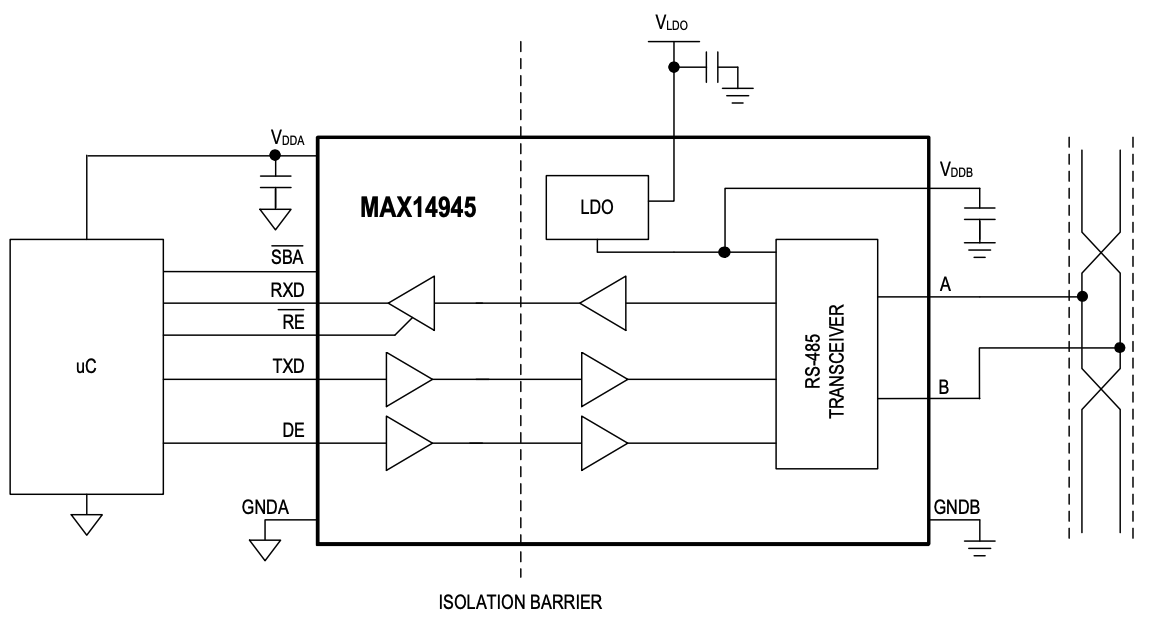
\includegraphics[width=.7\linewidth]{MAX_typical}
		\caption{MAX14945EWE+ Typical Application Circuit \cite[s.19]{MAX14945MN}}
		\label{fig:MAXfd}
	\end{center}
\end{figure}
Abbildung \ref{fig:MAXfd} zeigt den schematischen Aufbau des Treiberchips inklusive dessen typischer Beschaltung. Im blau markierten Bereich befindet sich die galvanische Trennung des Chips. Die gestrichelte Linie in der Mitte markiert die Trennung der Seiten $A$ und $B$. Die Funktionen der Pins können Tabelle \ref{tab:MAX_pins} entnommen werden. Die linke Seite ($A$ Seite) ist dem Mikrocontroller zugewendet und wird mit dem 5\,V Potential der USB-Schnittstelle versorgt und mit einem 0,1\,$\mu$F und 1\,$\mu$F Kondensator in Parallelschaltung gestützt. Die Kondensatoren sollen laut Datenblatt möglicht nah am Treiberchip platziert werden. Pin $TXD$ wird mit dem Ausgang, Pin $RXD$ mit dem Eingang der UART-Schnittstelle des MCUs verbunden. Zum aktivieren des Senders oder Empfängers des Treibers muss ein entsprechender Logikpegel an den Pins $DE$ und $\overline{RE}$ anliegen. Da die Logik des Pins zum aktivieren und deaktivieren des Empfängers invertiert ist, können beide Pins kurzgeschlossen werden und mit einem Ausgang des MCUs verbunden werden. Ein interner pulldown-Widerstand an beiden Pins ermöglicht die direkte Verbindung zum MCU ohne weitere Beschaltung. Die rechte Seite ($B$ Seite) des Treiberchips muss um die galvanische Trennung zu gewährleisten mit einer entsprechend getrennten Spannungsquelle versorgt werden. Diese wird mithilfe eines DC/DC Konverters, der die von der USB-Schnittstelle eingehenden 5\,V isoliert und am Ausgang wieder ausgibt \cite{DC_MN}. Um eine möglichst stabile Spannungsquelle zu gewährleisten wird der im Treiberchip interne $low-dropout$-Spannungsregler vewendet, wodurch Pin $V_{DDB}$ als Ausgang der stabilisierten Spannung fundiert. Pin $V_{DDB}$ und $V_{LDO}$ werden mit jeweils einem 0,1\,$\mu$F und parallegeschlaltetem 1\,$\mu$F Kondensator mit $GNDB$ verbunden.
\begin{table}[h]
	\begin{center}
		\begin{tabular}{l | l}
			\textbf{Pin} & \textbf{Funktion}\\
			\hline
			$TXD$ & serieller Dateneingang\\
			$RXD$ & serieller Datenausgang\\
			$DE$ & 1: Sender aktivieren, 0: Sender deaktivieren\\
			$\overline{RE}$ & 1: Empfänger deaktivieren, 0: Empfänger aktivieren\\
			$\overline{SBA}$ & 1: $B$ Seite inaktiv, 0: $B$ Seite funktionsfähig\\
			$A$ \& $B$ & symmetrischer Treiberausgang\\
			$V_{DDA}$ \& $GNDA$ & Spannungsversorgung $A$ Seite\\
			$V_{DDB}$ \& $GNDB$ & Spannungsversorgung $B$ Seite\\
			$V_{LDO}$ & Spannungsregler Eingang $B$ Seite
		\end{tabular}
	\caption{Pinbeschreibung MAX14945EWE+ \cite[s.12-13]{MAX14945MN}}
	\label{tab:MAX_pins}
	\end{center}
\end{table}
%Abbildung \ref{fig:MAXfd} zeigt den schematischen Aufbau des Treiberchips. Die gestrichelte Linie zeigt die galvanische Trennung im inneren des ICs. Auf der linken Seite ($A$ Seite) befindet sich der serielle Eingang ($TXD$) und Ausgang ($RXD$) sowie die Pins $DE$ zum aktivieren und $\overline{$$RE$} deaktivieren des Treibers. Der invertierte Ausgang $\overline{SBA}$ gibt einen low-Pegel aus wenn die rechte Seite (B-Seite) des ICs mit Spannung versorgt ist und funktioniert. Der eigentliche Treiber, sowie dessen symmetrischer Ein- und Ausgang ($A$ und $B$) befinden sich auf Seite $B$. Außerdem finden sich insgesamt 5\,Pins für die Spannungsversorgung des ICs. Um eine vollständige galvanisch entkopplung zu garantieren muss die Spannungsversorgung der $A$ und $B$ Seite auch galvanisch entkoppelt sein. Aus diesem Grund gibt es zwei Pin-Paare, bestehend aus $VDD$ \& $GND$, für Seite $A$ und $B$. Zusätzlich steht auf Seite $B$ ein interner \textit{low-dropout} Spannungsregler (LDO\footnote{Hochempfindliche Schaltung zur linearen Regelung einer spezifischen Spannung. \cite{LDO}}) zur Versorgung der Seite $B$ zur Verfügung. Die galvanisch entkoppelte Spannungsversorgung wird mithilfe eines DC/DC-Konverters mit 5\,V Ein- und Ausgang erreicht. Gespeist wird der Konverter direkt von der USB-Buchse. Seite $B$ benötigt eine Versorgungsspannung zwischen 4,68\,V und 14\,V zwischen Pin $VLDO$ und $GNDB$, Seite $A$ eine Spannung zwischen 1,71\,V und 5,5\,V zwischen Pin $VDDA$ und $GNDA$ \cite[s. 2]{MAX14945MN}. Um Stromspitzen und den damit einhergehenden mögichen Spannungseinbruch aufzufangen werden jeweils zwei Stützkondensatoren mit einer Kapaität von 100\,nF und 1\,$\mu$F zwischen den Versorgungspins geschaltet. 
%-Preistechnis kein Nachteil gegenüber einzelnem Treiber und Optokopplern\\
%-Galvanisch getrennte Spannungsversorgung nach wie vor notwendig\\